\documentclass{sig-alternate}
\usepackage[latin1]{inputenc}
\usepackage{graphicx}        % standard LaTeX graphics tool
\usepackage{url} 

\providecommand{\e}[1]{\ensuremath{\times 10^{#1}}}
\begin{document}
%
% --- Author Metadata here ---
\conferenceinfo{GECCO'13,} {July 6-10, 2013, Amsterdam, The Netherlands.}
    \CopyrightYear{2013}
    \crdata{TBA}
    \clubpenalty=10000
    \widowpenalty = 10000

\title{Effect of population size in heterogeneous and homogeneous machines in a distributed EA}

%\subtitle{[Extended Abstract]
%\titlenote{A full version of this paper is available as
%\textit{Author's Guide to Preparing ACM SIG Proceedings Using
%\LaTeX$2_\epsilon$\ and BibTeX} at
%\texttt{www.acm.org/eaddress.htm}}}
%
% You need the command \numberofauthors to handle the 'placement
% and alignment' of the authors beneath the title.
%
% For aesthetic reasons, we recommend 'three authors at a time'
% i.e. three 'name/affiliation blocks' be placed beneath the title.
%
% NOTE: You are NOT restricted in how many 'rows' of
% "name/affiliations" may appear. We just ask that you restrict
% the number of 'columns' to three.
%
% Because of the available 'opening page real-estate'
% we ask you to refrain from putting more than six authors
% (two rows with three columns) beneath the article title.
% More than six makes the first-page appear very cluttered indeed.
%
% Use the \alignauthor commands to handle the names
% and affiliations for an 'aesthetic maximum' of six authors.
% Add names, affiliations, addresses for
% the seventh etc. author(s) as the argument for the
% \additionalauthors command.
% These 'additional authors' will be output/set for you
% without further effort on your part as the last section in
% the body of your article BEFORE References or any Appendices.


\numberofauthors{2}
 \author{
 \alignauthor
 Anonymous\\
        \affaddr{Lost island}\\
        \affaddr{Unknown}\\
        \affaddr{Pacific Ocean}\\
        \email{jack,sawyer,hurley@lost.com}
 \alignauthor
 Anonymous\\
 \affaddr{Lost island}\\
 \affaddr{Unknown}\\
 \affaddr{Pacific Ocean}\\
 \email{lock@lost.com}
 }

%\numberofauthors{2}
% \author{
% \alignauthor
% J.J. Merelo, A.M. Mora, C. M. Fernandes\\
%        \affaddr{University of Granada}\\
%        \affaddr{Department of Computer Architecture and Technology, ETSIIT}\\
%        \affaddr{18071 - Granada}\\
%        \email{jmerelo,amorag,cfernandes@geneura.ugr.es}
% \alignauthor
% Anna I. Esparcia-Alcázar\\
% \affaddr{S2 Grupo}\\
% \email{aesparcia@s2grupo.es}
% }


%\numberofauthors{4} %  in this sample file, there are a *total*
% of EIGHT authors. SIX appear on the 'first-page' (for formatting
% reasons) and the remaining two appear in the \additionalauthors section.
%

%\author{
% You can go ahead and credit any number of authors here,
% e.g. one 'row of three' or two rows (consisting of one row of three
% and a second row of one, two or three).
%
% The command \alignauthor (no curly braces needed) should
% precede each author name, affiliation/snail-mail address and
% e-mail address. Additionally, tag each line of
% affiliation/address with \affaddr, and tag the
% e-mail address with \email.
%
% 1st. author
%\alignauthor
%Jack\\
%       \affaddr{Lost island}\\
%       \affaddr{unknow}\\
%       \affaddr{Pacific Ocean}\\
%       \email{jack_the_doctor@lost.com}
% 2nd. author
%\alignauthor
%Sawyer\\
%       \affaddr{Lost island}\\
%       \affaddr{unknow}\\
%       \affaddr{Pacific Ocean}\\
%       \email{sawyer_tom@lost.com}
% 3rd. author
%\alignauthor 
%Lock\\
%       \affaddr{Lost island}\\
%       \affaddr{unknow}\\
%       \affaddr{Pacific Ocean}\\
%       \email{lock@lost.com}
% 4rd. author
%\alignauthor 
%Hurley\\
%       \affaddr{Lost island}\\
%       \affaddr{unknow}\\
%       \affaddr{Pacific Ocean}\\
%       \email{hugo@lost.com}
%}

%\and  % use '\and' if you need 'another row' of author names
% 4th. author
%\alignauthor Lawrence P. Leipuner\\
%       \affaddr{Brookhaven Laboratories}\\
%       \affaddr{Brookhaven National Lab}\\
%       \affaddr{P.O. Box 5000}\\
%       \email{lleipuner@researchlabs.org}
% 5th. author
%\alignauthor Sean Fogarty\\
%       \affaddr{NASA Ames Research Center}\\
%       \affaddr{Moffett Field}\\
%       \affaddr{California 94035}\\
%       \email{fogartys@amesres.org}
% 6th. author
%\alignauthor Charles Palmer\\
%       \affaddr{Palmer Research Laboratories}\\
%       \affaddr{8600 Datapoint Drive}\\
%       \affaddr{San Antonio, Texas 78229}\\
%       \email{cpalmer@prl.com}
%}
% There's nothing stopping you putting the seventh, eighth, etc.
% author on the opening page (as the 'third row') but we ask,
% for aesthetic reasons that you place these 'additional authors'
% in the \additional authors block, viz.
%\additionalauthors{Additional authors: John Smith (The Th{\o}rv{\"a}ld Group,
%email: {\texttt{jsmith@affiliation.org}}) and Julius P.~Kumquat
%(The Kumquat Consortium, email: {\texttt{jpkumquat@consortium.net}}).}
%\date{30 July 1999}
% Just remember to make sure that the TOTAL number of authors
% is the number that will appear on the first page PLUS the
% number that will appear in the \additionalauthors section.

\maketitle

\begin{abstract}
This paper shows a preliminary study about population size tuning in an distributed genetic algorithm. This adaptation is done taking into account the computational power of each node of an heterogeneous cluster. Two problems with distinct characteristics have been tested: the linearly-solvable OneMax problem and the deceptive and multimodal MMDP functions. Same parameters are also tested in an homogeneous scientific cluster. Results show that setting this parameter according computational power decreases the time to obtain the optimum in both problems in heterogeneous clusters.
\end{abstract}

% A category with the (minimum) three required fields
\category{H.4}{Information Systems Applications}{Miscellaneous}
%A category including the fourth, optional field follows...
\category{G.1.6}{Mathematics of Computing}{NUMERICAL ANALYSIS}[Optimization]


%sures, performance measures
\terms{Algorithms}


\keywords{parameter setting, distributed algorithms, island model}


%
%%%%%%%%%%%%%%%%%%%%%%%%%%%%%%%   INTRODUCTION   %%%%%%%%%%%%%%%%%%%%%%%%%%%%%%%
%
\section{Introduction}
\label{sec:intro}
%
New trends such as Cloud Computing \cite{CLOUD}, GRID \cite{OPENSCIENCEGRID} or Service Oriented Science \cite{GLOBUS} are leading to heterogeneous computational devices working at the same time.  Moreover, many laboratories do not count with classic clusters, but the usual workstations used by scientists can behave in group as a heterogeneous cluster. Distributed Evolutionary Algorithms (dEAs) have been tested in these systems with SUCCES?. These systems can take advantage of heterogeneous dEAs. 

Heterogeneous dEAs can be divided in two categories: a dEA where the parameters are different in each island (heterogeneous parameters) or the same algorithm in heterogeneous hardware. It also have been proved that this kind of algorithms are even more efficient in heterogeneous hardware configurations, than in homogeneous devices \cite{HETEROGENEOUSHARD}. This can be explained by different reasons, such as different memory access times, cache, or even implementation languages or compilers in each machine, leading to different explotation rate of the search space. The heterogeneous parameters configuration also have been proved as more efficient than a fixed set of parameters for different problems \cite{HETEROGENEOUSPARAMETERS}. Our motivation in this work is to combine both ideas adapting the population size of the islands to the heterogeneous hardware. To calculate the computational power, the algorithm is executed in each machine and distribute a total size of individuals according the number of generations attained in each node during the same time. Two different problems (MMDP and OneMax) have been used as a benchmark.


In this work, a distributed system has been developed to solve the following questions:
\begin{itemize}
 \item Can a distributed EA be adapted to take the most of the performance of a heterogeneous cluster?
 \item Does the proposed population size adaptation to the computational power scheme any effect in both systems?
 \item Is there any difference in homogeneous and heterogeneous clusters?
\end{itemize}


The rest of the work is structured as follows: after the state of
the art, we present the developed algorithms and experimental setting. 
Then, the results of the experiments are shown (Section \ref{sec:results}), followed by conclusions and suggestions for future work.


%%%%%%%%%%%%%%%%%%%%%%%%%%%%%%  SOA  %%%%%%%%%%%%%%%%%%%%%%%%%%%%%%
%
\section{State of the art}
\label{sec:soa}
%

In the field of the Evolutionary Computing there are two different approaches about the algorithm parameter setting: parameter control and parameter tuning \cite{PARAMETERTUNING}. The first one refers to set a number of parameters of an EA and change these parameter while the algorithm is running. The parameter tuning consist in establish a good set of parameters before the run (and do not change them during runtime).

 In \cite{HETEROGENEOUSHARD} authors compare a distributed GA in homogeneous and heterogeneous clusters. Super-linear performance is obtained in the heterogeneous clusters, being more efficient that the same algorithm in homogeneous clusters. Some authors have expanded this idea adapting the algorithm to be executed: in \cite{HYDROCM} a distributed meta-heuristic executes simpler algorithms in simpler nodes. In \cite{HETEROGENEOUSTOPOLOGY} different configurations of heterogeneous machines for a tree topology are studied. However, the heterogeneity is simulated in an homogeneous clusters. Load-balancing is also applied taking into account the computational load of the nodes in \cite{PARALLELIMPLEMENTATION}: a small benchmark is executed in all nodes at the start of the algorithm to distribute individuals of an Evolutionary Strategy (ES). However, there is not communication between the nodes. In the area of heterogeneous parameters, but homogeneous hardware, setting each island a random set of parameters can also increase the performance of a distributed Genetic Algorithm (dGA), as explained in \cite{HETEROGENEOUSPARAMETERS}. That model outperformed a tuned canonical dGA with the same parameters in all islands. Finally, adapting the migration period have been produced better results than homogeneous periods in homogeneous cluster, as claimed by \cite{HETEROGENEOUSMIGRATION}.

 Our work presents a combination of previous ideas, where a parameter tuning given by the computational cost of the machines is performed. For our knowledge, there are not works that modify parameters of the GA depending of the node where the island is being executed.

%%%%%%%%%%%%%%%%%%  Experiments  %%%%%%%%%%%%%%%%%%%

\section{Experimental setup}
\label{subsec:experiments}
This section presents the parameters and systems to conduce the experiments.

The algorithm to improve is a distributed Genetic Algorithm (dGA). Parameters are described in Table \ref{table:parameters}. The algorithm is steady-state: the offspring is mixed with the parents and the worst individuals are removed. A ring topology has been used, and the best individual is sent after a fixed number of generations.  Two different parameter configurations have been used: 64 individuals per node (homogeneous size) and a different number of individuals proportional to the number of generations attained in this first homogeneous size execution (heterogeneous size).


\begin{table}
\centering
\caption{Parameters used.}
\begin{tabular}{|c|c|} \hline
Name & Value\\ \hline
Total individuals & 256\\ \hline
Population size in HoSi & 64 \\ \hline
Population size in HeSi & 98, 84, 66, and 8\\ \hline
Crossover type & Uniform crossover \\ \hline
Crossover rate & 0.5\\ \hline
Mutation rate & 1/genome size\\ \hline
Selection & 2-tournament \\ \hline
Replacement & Steady-state\\ \hline
Generations to migrate & 64 \\ \hline
Genome size for MMDP & 150 \\ \hline
Genome size for OneMax & 5000 \\ 

\hline\end{tabular}
\label{table:parameters}
\end{table}

The problems to evaluate are the Massively Multimodal Deceptive Problem (MMDP) \cite{goldberg92massive} and the OneMax problem \cite{ONEMAX}. Each one requires different actions/abilities by the GA at the level of population sizing, individual selection and building-blocks mixing. The MMDP
 is designed to be difficult for an EA, due to
its multimodality and deceptiveness. Deceptive problems are functions where low-order building-blocks do not combine to form higher order building-blocks. Instead, low-order building-blocks may mislead the search towards local optima, thus challenging search mechanisms. MMDP it is composed of $k$ subproblems of 6 bits each one ($s_i$). Depending of
the number of ones (unitation) $s_i$ takes the values shown in Table \ref{table:mmdp}.  

\begin{table}[h]

\centering
{%\scriptsize
\caption{ Basic deceptive bipolar function ($s_i$) for MMDP.}
\begin{tabular}{|c|c|}
\hline
\texttt{Unitation}&\texttt{Subfunction value}\\
\hline
0 & 1.000000 \\
\hline
1 & 0.000000 \\
\hline
2 & 0.360384 \\
\hline
3 & 0.640576\\
\hline
4 & 0.360384\\
\hline
5 & 0.000000\\
\hline
6 & 1.000000\\
\hline

\end{tabular}
}

\label{table:mmdp}
\end{table}
%%%%%%%%%%%%%%%%%%



The fitness value is defined as the sum of the $s_i$ subproblems with an optimum of $k$ (equation \ref{eq:mmdp}).
The search space is composed of $2^{6k}$ combinations from which there
are only $2^k$ global solutions with $22^k$ deceptive
attractors. Hence, a search method will have to find a global solution
out of $2^{5k}$ additionally to deceptiveness. In this work $k=25$. 

\begin{equation}\label{eq:mmdp}
\scriptsize
f_{MMDP}(\vec s)= \sum_{i=1}^{k} fitness_{s_i}
\end{equation}\\

Onemax is a simple linear problem that consists in maximising the number of ones in a binary string. That is, maximize the expression:
\begin{equation}
f_{OneMax}(\vec{x}) = \sum_{i=1}^{N}{x_{i}}
\end{equation}


To test the algorithm two different computational systems have been used: an {\em heterogeneous cluster} and an {\em homogeneous cluster}. The first one is formed by 4 different computers of our lab with different processors, operating systems and memory. The latter is a dedicated scientific cluster formed by homogeneous nodes. Table \ref{tab:computers} shows the features of each system.

\begin{table*}
\centering{\scriptsize
\caption{Details of the clusters used.}
\begin{tabular}{|c|c|c|c|c|} \hline
Name 		 & Processor 	& Memory 	& Operating System  & Network  \\ \hline
\multicolumn{5}{|c|}{Homogeneous cluster} \\ \hline
Cluster node &	Intel(R) Xeon(R) CPU   E5320  @ 1.86GHz		    &	4GB	& CentOS 6.7		& 	??  	\\ \hline
\hline
\multicolumn{5}{|c|}{Heterogeneous cluster} \\ \hline
N1	&	 Intel(R) Core(TM)2 Quad CPU    Q6600  @ 2.40GHz		& 4GB		&	Ubuntu 11.10 (64 bits)	&	Gigabit Ethernet	  	\\ \hline
N2 	&	 Intel(R) Core(TM)2 Quad CPU    Q6600  @ 2.40GHz		& 4GB		&	Ubuntu 11.04 (64 bits)	&	?? Ethernet	  	\\ \hline
N3 	&	 AMD Phenom(tm) 9950 Quad-Core Processor @ 1.30Ghz		& 3GB		&	Ubuntu 10.10 (32 bits)	&	?? Ethernet	  	\\ \hline
N4 	&	 Intel (R) Pentium 3 @ 800MHz		    				& 768 MB	&	Ubuntu 10.10 (32 bits)	& 		  	\\ \hline
\end{tabular}
}
\label{tab:computers}
\end{table*}

Because the operating system and architecture heterogeneity the ANONYMOUS framework \cite{OSGILIATH}, based in Java, has been used. This is a service-oriented evolutionary framework that automatically configures services to use and be used in a local network. In this case, each node offers a migration buffer to accept foreign individuals. Also, to avoid bottlenecks in distributed executions, asynchronous communication has been provided to avoid idle time using reception buffers (that is, the algorithm does not wait until new individuals arrive). This kind of communication offers excellent performance when working with different nodes and operating systems, as demonstrated by \cite{HETEROGENEOUSHARD}. The transmission mechanism is based in ECF Generic server (over TCP) \footnote{\url{http://www.eclipse.org/ecf/}}. The source code of the algorithms used in this work is available in \url{http://anonymous} under a GPL V3 License.

Each different configuration has been tested 30 times. Acronyms for each configuration are HoSi (homogeneous population size), HeSi (heterogeneous population size), HoHa (homogeneous hardware) and HeHa (heterogeneous hardware). The population sizes are obtained after the execution of the HoSi/HeHa version of the MMDP and divide the total number of individuals (256) proportional to the average number of generations attained in each node. Thus, the HeSi configuration uses 98, 84, 66, and 8 individuals (from N1 to N4). Note that, having two nodes with the same processors and memory (N1 and N2), they have different computational power.
%%%%%%%%%%%%%%%%%%  Results  %%%%%%%%%%%%%%%%%%%

\section{Results}
\label{sec:results}

As claimed by \cite{EVALUATIONPARALLEL} the number of evaluations can be misleading in the parallel algorithms area. In our case, for example, the evaluation time is different in each node of the heterogeneous cluster, and the real algorithm speed could not be reflected correctly. Also, the main interest in parallel programming is to reduce time. However, the number of evaluations has been added for comparison between the results of the HoHa system. It is difficult to compare between the HoHa and HeHa for the same reasons: the evaluation time is different in each system (and machine) ESTO DEBERIA JUSTIFICARLO MAS.

\subsection{MMDP Problem}

Table \ref{tab:resultsMMDP} shows the results for the MMDP problem. These results are also show in the boxplots of the Figure \ref{fig:evalsMMDP} (evaluations) and Figure \ref{fig:timeMMDP} (time). Table \ref{tab:significance} shows the statistical significance of the results. First, a Kolmogorov-Smirnov test is performed to asset the normality of the distributions. If the results are normal, then a Student's T-Test is run. Otherwise, the non-parametric test Wilcoxon signed rank is applied (see \cite{TUTORIAL} for a tutorial for comparing EAs).

 In the HeHa system, adapting the population to the computational power of each nodes makes the algorithm to end faster, but with the same number of evaluations (no statistical significance). This can be explained because the evaluation time is different in all nodes. On the other hand, in the HoHa system, setting the same population sizes makes no difference in time and evaluations. EXPLICAR.

\begin{table*}
\centering
\caption{Results for the MMDP problem.}
\begin{tabular}{|c|c|c|c|c|} \hline
Configuration	& Max. generations			& Total generations			& 	Total evaluations			& Time (ms) \\ \hline
HoSi/HeHa		& 146401,48	$\pm$ 65699,69	& 380967,25	$\pm$ 168568,84	& 24382416,51 $\pm$	10788405,87	& 136914,03 $\pm$ 60028,48\\ \hline
HeSi/HeHa		& 96051,5	$\pm$ 45110,90	& 289282,3	$\pm$ 135038,10	& 21784528,66 $\pm$	10161989,38	& 109875,76 $\pm$ 49185,51\\ \hline \hline
HoSi/HoHa		& 107334,46 $\pm$ 78167,19  & 393119,86 $\pm$ 241835,27	& 25273201,06 $\pm$ 15386663,12	& 237759,43 $\pm$ 178709,86\\ \hline
HeSi/HoHa		& 149732,6 $\pm$ 81983,74	& 438171,16	$\pm$ 240169,19	& 24430043,46 $\pm$ 13395037,34	& 245776,93 $\pm$ 134715,52\\ \hline

\end{tabular}
\label{tab:resultsMMDP}
\end{table*}
%%%%CAMBIAR EL ORDEN!!!

%MMDP EVALS
%HomoSizeHomoHard-HomoSizeHeteroHard 22.83333     23.69541      FALSE
%HomoSizeHomoHard-HeteroSizeHomoHard  4.90000     23.69541      FALSE
%HomoSizeHomoHard-HeteroSizeHeteroHard 37.53333     23.69541       TRUE
%HomoSizeHeteroHard-HeteroSizeHomoHard 27.73333     23.69541       TRUE
%HomoSizeHeteroHard-HeteroSizeHeteroHard 14.70000     23.69541      FALSE
%HeteroSizeHomoHard-HeteroSizeHeteroHard 42.43333     23.69541       TRUE





\begin{figure}
\centering
\epsfig{file=images/timeMMDP.eps, width = 9cm}
\caption{Time to obtain the optimum in the MMDP problem (milliseconds). White is the heterogeneous cluster and gray the homogeneous one.}
\label{fig:timeMMDP}
\end{figure}

\begin{figure}
\centering
\epsfig{file=images/evalsMMDP.eps, width = 9cm}
\caption{Number of evaluations for MMDP problem. White is the heterogeneous cluster and gray the homogeneous one.}
\label{fig:evalsMMDP}
\end{figure}

To see the difference of how the evolution is being performed, the average fitness in each node of HeHa is shown in Figures \ref{fig:hosiheha} and \ref{fig:hesiheha}. As can be seen, with the HeSi (Figure \ref{fig:hesiheha}), the local optima are overtaken in less time than HoSi (Figure \ref{fig:hosiheha}). This can be explained because in HeSi, the migration from N4 to N1 is performed faster, adding more heterogeneity to the whole system. In the HoHa systems, the populations are evolved at the same time, being the average fitness similar in all nodes during all run. % The natural migration period variation from a processor to another is also giving more diversity to the populations that migrating at the same time of the homogeneous



\begin{figure}
\centering
\epsfig{file=images/heterosize_heterohard_avg.eps, angle=-90, width = 9cm}
\caption{Average fitness in the first 1000 milliseconds of execution of the four nodes of the heterogeneous cluster with different population sizes (MMDP problem).}
\label{fig:hesiheha}
\end{figure}

\begin{figure}
\centering
\epsfig{file=images/homosize_heterohard_avg.eps, angle=-90, width = 9cm}
\caption{Average fitness in the first 1000 milliseconds of execution of the four nodes of the heterogeneous cluster with the same population sizes (MMDP problem).}
\label{fig:hosiheha}
\end{figure}

\subsection{OneMax Problem}

Results for this problem are shown in Table \ref{tab:onemaxresults} and Figures \ref{fig:evalsOneMax} and \ref{fig:timeOneMax}. As before, in this problem, changing the population sizes decreases significantly the time  in the heterogeneous cluster, and also the number of evaluations remains the same (see statistical significance in Table \ref{tab:significance}). In the homogeneous system, the effect of changing this sizes is more evident, and this time the evaluations (and therefore, the time) are reduced (both significally). 

The efficiency on OneMax problems depends more on the ability to mix the building-blocs, and less on the genetic diversity and size of the population (as with MMDP). No genetic diversity is particularly required. When properly tuned, a simple Genetic Algorithm is able to solve OneMax in linear time. Sometimes, problems like OneMax are used as control functions, in order to check if very efficient algorithms on hard functions fail on easier functions. As can be seen in Figure \ref{fig:gensonemaxhomosize}, the HoSi/HeHa, the average fitness of all populations are increasing in linear way. However, the lower processor evaluates extremely less times.  On the other side, in Figure \ref{fig:gensonemaxheterosize}, the adaptation of the population size makes that lower processors increase the number of evaluations, but the average fitness is also maintained in linear way (and in smaller increase rate). However, the other processors are still spending more number of evaluations. That is the reason why the number of evaluations is higher in HeHa, and lower in HoHa. Computational time is more efficiently used in faster processor, having more chance to mix the individuals. Also, because the larger size of the individuals in the OneMax problem (5000 bits vs. 150), the transmission time is larger (white gaps in the figures). That also implies for N4 send their best individual to N1 in a extremely large time when using HoSi (each 64 generations).

\begin{table*}
\centering
\caption{Results for the OneMax problem.}
\begin{tabular}{|c|c|c|c|c|} \hline
Configuration	& Max. generations			& Total generations			& 	Total evaluations			& Time (ms) \\ \hline
HoSi/HeHa		& 4739,41$\pm$	305,32 		&	12081,51$\pm$	776,35 	&	773729,03$\pm$	49686,72 	&	72152,32$\pm$	4994,71 \\ \hline
HeSi/HeHa		&	3438,03 $\pm$	149,47 &	11277,33$\pm$	471,77 &	794157,73$\pm$	31843,10 	&	61870,2	$\pm$ 2518,74 \\ \hline
HoSi/HoHa		&	3133,36$\pm$	101,70 	&	12347,83$\pm$	394,99 	&	790773,33$\pm$	25279,52 	&	62105,03$\pm$	1964,75 \\ \hline
HeSi/HoHa		& 13897,86$\pm$	625,27 		&	20725,63$\pm$	929,43 	&	651952,8 $\pm$	29114,54	&	56120,53$\pm$	2491,92 \\ \hline
\end{tabular}
\label{tab:onemaxresults}
\end{table*}

\begin{figure}
\centering
\epsfig{file=images/evalsOneMax.eps, width = 9cm}
\caption{Number of evaluations for OneMax problem. White is the heterogeneous cluster and gray the homogeneous one.}
\label{fig:evalsOneMax}
\end{figure}

\begin{figure}
\centering
\epsfig{file=images/timeOneMax.eps, width = 9cm}
\caption{Time to obtain the optimum in the OneMax problem (milliseconds). White is the heterogeneous cluster and gray the homogeneous one.}
\label{fig:timeOneMax}
\end{figure}

\begin{figure}
\centering
\epsfig{file=images/homosize_heterohard_onemax_avg.eps, angle=-90, width = 9cm}
\caption{Average fitness in the first 3000 milliseconds of execution of the four nodes of the heterogeneous cluster with the same population sizes (OneMax problem).}
\label{fig:gensonemaxhomosize}
\end{figure}

\begin{figure}
\centering
\epsfig{file=images/heterosize_heterohard_onemax_avg.eps, angle=-90, width = 9cm}
\caption{Average fitness in the first 3000 milliseconds of execution of the four nodes of the heterogeneous cluster with different population sizes (OneMax problem).}
\label{fig:gensonemaxheterosize}
\end{figure}

\begin{table*}
\centering
\caption{Statistical significance of the results.}
\begin{tabular}{|c|c|c|c|c|} \hline

Configuration			&Normal	&Test applied			&P-value & Significant difference?\\ \hline
\multicolumn{5}{|c|}{Time for MMDP} \\ \hline
HoSi/HeHa vs HeSi/HeHa	&Yes	&T-Test			& \textbf{0.032} 	 & Yes \\ \hline
HoSi/HoHa vs HeSi/HoHa	&No		&Wilcoxon		&0.567 	 & No \\ \hline
\multicolumn{5}{|c|}{Evaluations for MMDP}	\\ \hline
HoSi/HeHa vs HeSi/HeHa	&Yes	&T-Test			&0.231  & No \\ \hline
HoSi/HoHa vs HeSi/HoHa	&No		&Wilcoxon		&0.958  & No \\ \hline
\multicolumn{5}{|c|}{Time for OneMax} \\ \hline
HoSi/HeHa vs HeSi/HeHa	& Yes	& T-Test		&  \textbf{9\e{-15}} & Yes \\ \hline
HoSi/HoHa vs HeSi/HoHa	& No	& Wilcoxon		& 	1\e{-6} & Yes \\ \hline
\multicolumn{5}{|c|}{Evaluations for OneMax}	\\ \hline
HoSi/HeHa vs HeSi/HeHa	& No	& Wilcoxon 		&	0.14 		& No\\ \hline
HoSi/HoHa vs HeSi/HoHa	& Yes	& T-Test		&	2*\e{-27}	& Yes \\ \hline
\end{tabular}
\label{tab:significance}
\end{table*}

%\begin{table}
%\centering
%\caption{Frequency of Special Characters}
%\begin{tabular}{|c|c|l|} \hline
%Non-English or Math&Frequency&Comments\\ \hline
%\O & 1 in 1,000& For Swedish names\\ \hline
%$\pi$ & 1 in 5& Common in math\\ \hline
%\$ & 4 in 5 & Used in business\\ \hline
%$\Psi^2_1$ & 1 in 40,000& Unexplained usage\\
%\hline\end{tabular}
%\end{table}


%\begin{figure}
%\centering
%\epsfig{file=fly.eps}
%\caption{A sample black and white graphic (.eps format).}
%\end{figure}
%
%\begin{figure}
%\centering
%\epsfig{file=fly.eps, height=1in, width=1in}
%\caption{A sample black and white graphic (.eps format)
%that has been resized with the \texttt{epsfig} command.}
%\end{figure}

%\begin{figure*}
%\centering
%\epsfig{file=flies.eps}
%\caption{A sample black and white graphic (.eps format)
%that needs to span two columns of text.}
%\end{figure*}


\section{Conclusions}
New trends, such as Cloud Computing or Service Oriented Architecture are providing a massively amount of heterogeneous computational devices. BLABLABLA This work shows a preliminary study about adapting the population size of an EA to computational power of different nodes in an heterogeneous cluster. Results show that adapting the population size decrease the execution time significantly in heterogeneous clusters, while changing this parameter in homogeneous clusters not always performs better. This is a promising start for adapting EAs to the computational power of each machine.

In future work a scalability study will be performed, with more computational nodes and larger problem instances. Also, other parameters such as migration rate or crossover probability will be adapted to the computational nodes. This studies will lead to automatic adaptation during runtime, whith different nodes entering or exiting in the topology during the algorithm execution or adapting to system load.


%ACKNOWLEDGMENTS are optional
\section{Acknowledgments}
This work has been supported in part %by FPU research grant AP2009-2942 and projects AmIVital (CENIT2007-1010), EvOrq (P08-TIC-03903), UGR PR-PP2011-5 and TIN2011-28627-C04-02.

%
% The following two commands are all you need in the
% initial runs of your .tex file to
% produce the bibliography for the citations in your paper.


%\bibliographystyle{abbrv} CAMBIAR!!!!!!
\bibliographystyle{plain}
\bibliography{heterogeneous}  % sigproc.bib is the name of the Bibliography in this case


\end{document}